\documentclass[11pt]{article}
\usepackage{fullpage}
\usepackage{setspace}
\usepackage{amsmath}
\usepackage{fancyvrb}
\usepackage{enumerate}
\usepackage{pgfplots}
\usepackage{graphicx}
\usepackage{float}
\usepackage{multirow}

\begin{document}
\noindent\large{Math 5365}\\
\large{Data Mining 1}\\
\large{Homework 4}\\
\large{Mary Barker}
\newline
\singlespace
\begin{Verbatim}
#Data Mining Hw 4
library(stats)

####################################################################
#1: creating exdata dataset
x <- runif(1800, 0, 20)
y <- runif(1800, 0, 20)

x = c(x, rnorm(400, 10, 2), rnorm(400, 5, 2), rnorm(400, 15, 2))
y = c(y, rnorm(400, 5, 2), rnorm(400, 15, 2), rnorm(400, 15, 2))
class = c(rep(0, 1800), rep(1, 1200))
exdata <-data.frame(x,y,class)

####################################################################
#2: problems a) through h)
#a) create scatterplot
plot(exdata$x, exdata$y, col=c("blue","green")[as.factor(class)])
\end{Verbatim}

\begin{figure}[H]
\begin{center}
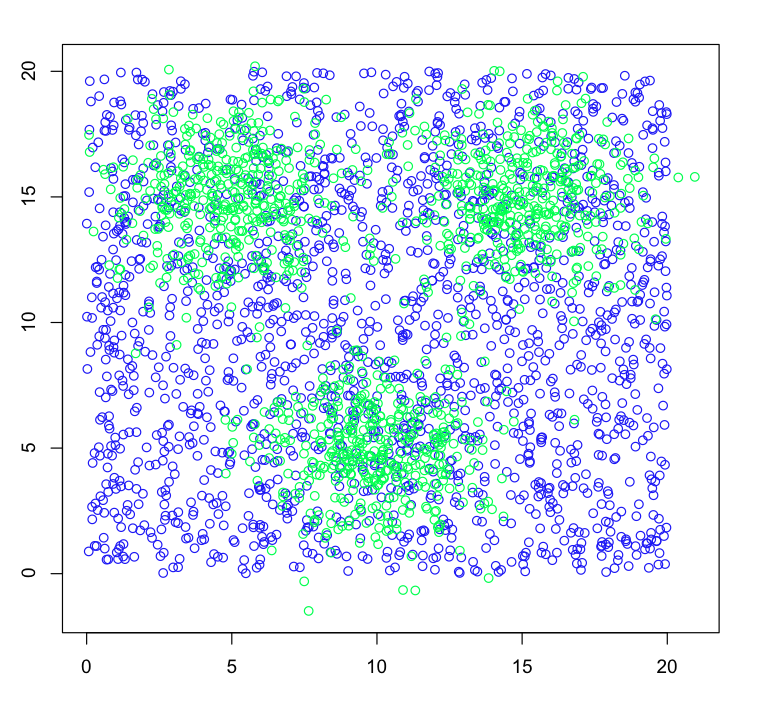
\includegraphics[scale=0.35]{images/scatter}
\caption{Problem 2 (a) scatterplot for exdata}
\end{center}
\end{figure}

\begin{Verbatim}
#b) split data into training set(30%) and test set(70%)
sz = nrow(exdata)
traindata = exdata[sample(nrow(exdata), 0.3 * sz),]
testdata <- exdata[which(!row.names(exdata) %in% row.names(traindata)), ]

#c) use rpart to fit a decision tree called extree to 
#   the training data and find the training data error 
#   and testing error for the tree. Also, plot extree 
#   with the plot command.
library(rpart)
library(rpart.plot)
library(party)
library(rattle)
library(treemap)

extree = rpart(as.factor(class)~x+y)
#prp(extree, type=1, extra=102)
fancyRpartPlot(extree)
\end{Verbatim}

\begin{figure}[H]
\begin{center}
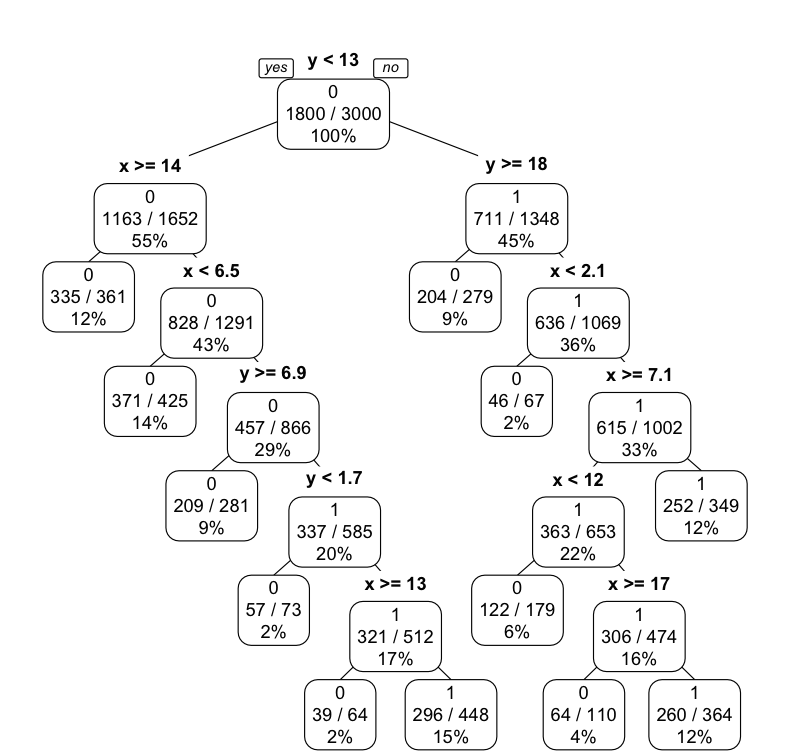
\includegraphics[scale=0.35]{images/extree_fancy}
\caption{Problem 2 (c) plot of extree }
\end{center}
\end{figure}

\begin{Verbatim}
pred_extree = predict(extree, newdata = traindata, type='class')
train_c_mat = table(traindata$class, pred_extree)
train_accuracy = sum(diag(train_c_mat)) / sum(train_c_mat)

pred_extree = predict(extree, newdata = testdata, type='class')
test_c_mat = table(testdata$class, pred_extree)
test_accuracy = sum(diag(test_c_mat)) / sum(test_c_mat)
\end{Verbatim}

In order to find the error for the training and testing predictions, 
the accuracy was subtracted from 1 to give a decimal representation. 
1 - train$\_$accuracy resulted in 
 0.2555556
Therefore the training error is approximately 26\%
.

1 - test$\_$accuracy resulted in 
0.2452381
And so the testing error is approximately 25 \%.
\begin{Verbatim}
#d) Construct trees with maxdepth = 1, 2, ... , 6. For each tree, store its
#      training error
#      test error
#      number of nodes
#   in a matrix

max_depth = seq(1, 6, 1)
train_error = rep(0, 6)
test_error = rep(0, 6)
n_nodes = rep(0, 6)
as.factor(testdata$class)

for (mdepth in 1:6){
	t_tree = rpart(as.factor(class)~x+y, 
	traindata, control = rpart.control(maxdepth = mdepth))
    plot(t_tree, main=c("max depth = ",mdepth))
    n_nodes[mdepth] = dim(t_tree$frame)[1]

    pred_t_tree = predict(t_tree, newdata = traindata, type='class')
    t_matrix = table(traindata$class, pred_t_tree)
    t_accuracy = sum(diag(t_matrix)) / sum(t_matrix)

    train_error[mdepth] = 1 - t_accuracy

    pred_t_tree = predict(t_tree, newdata = testdata, type='class')
    t_matrix = table(testdata$class, pred_t_tree)
    t_accuracy = sum(diag(t_matrix)) / sum(t_matrix)

    test_error[mdepth] = 1 - t_accuracy
}
ctrl1 <-data.frame(max_depth, train_error, test_error, n_nodes)
\end{Verbatim}

\begin{center}

\includegraphics[scale=0.25]{images/mdepth=1}
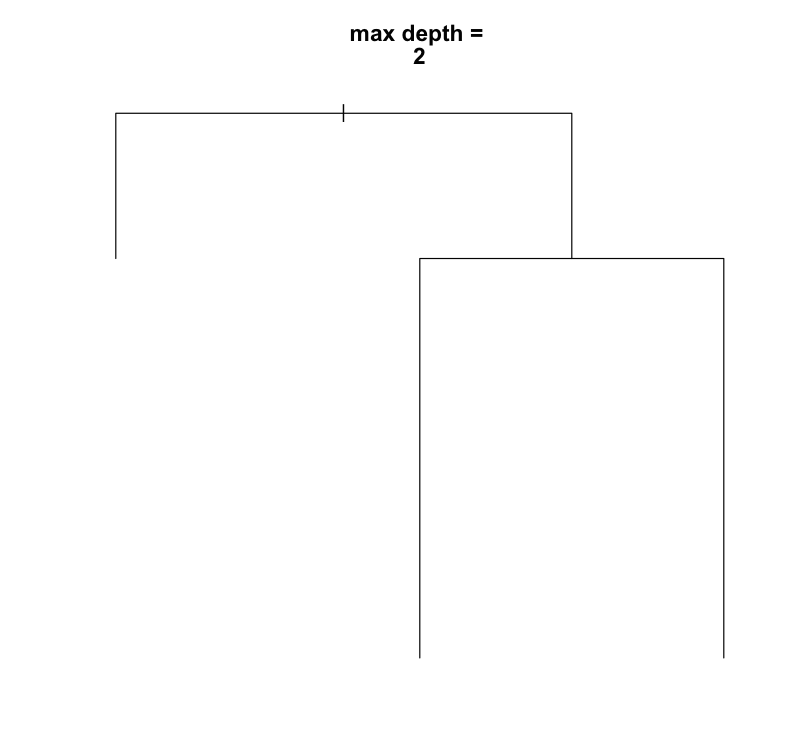
\includegraphics[scale=0.25]{images/mdepth=2}
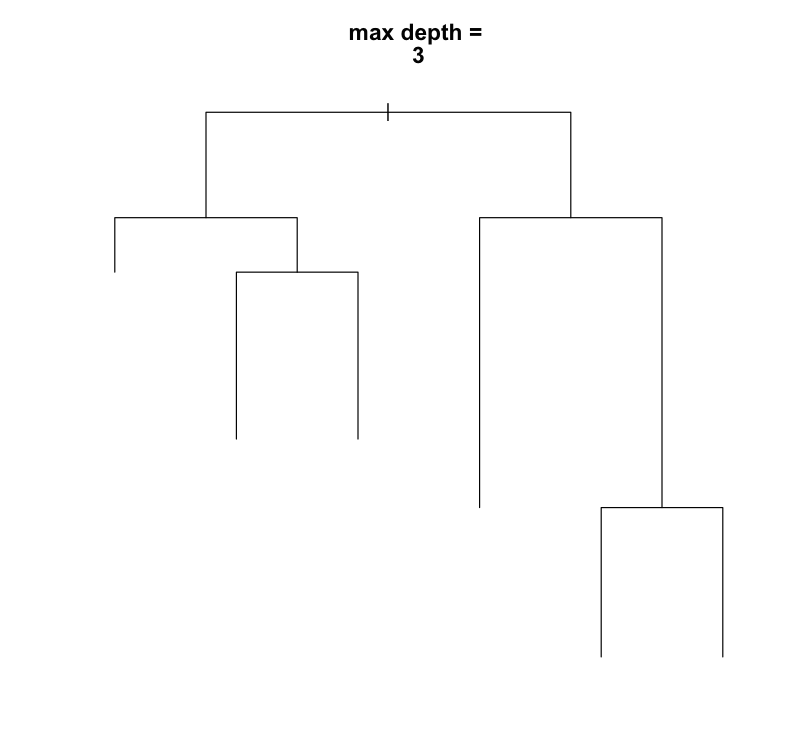
\includegraphics[scale=0.25]{images/mdepth=3}
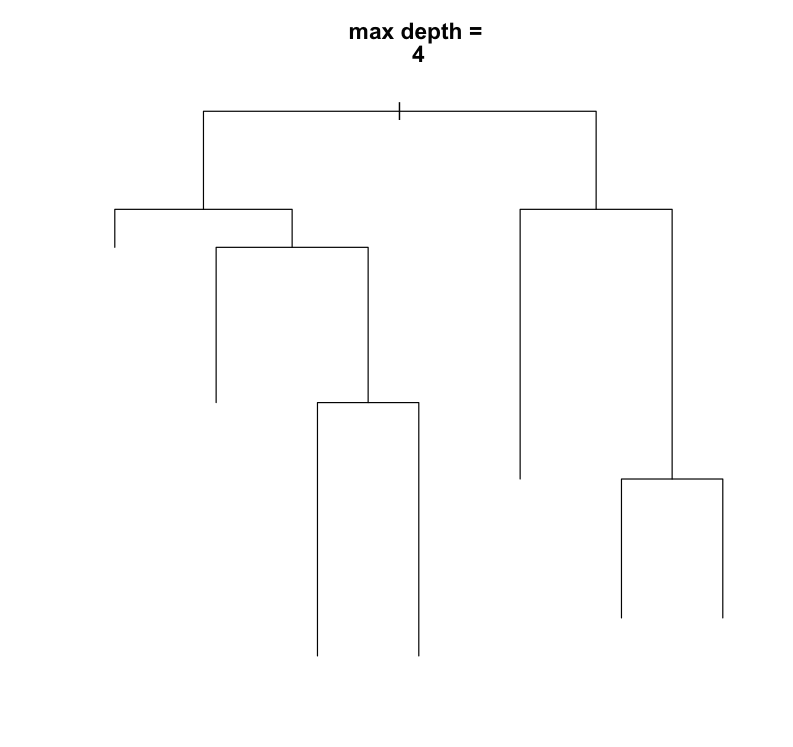
\includegraphics[scale=0.25]{images/mdepth=4}
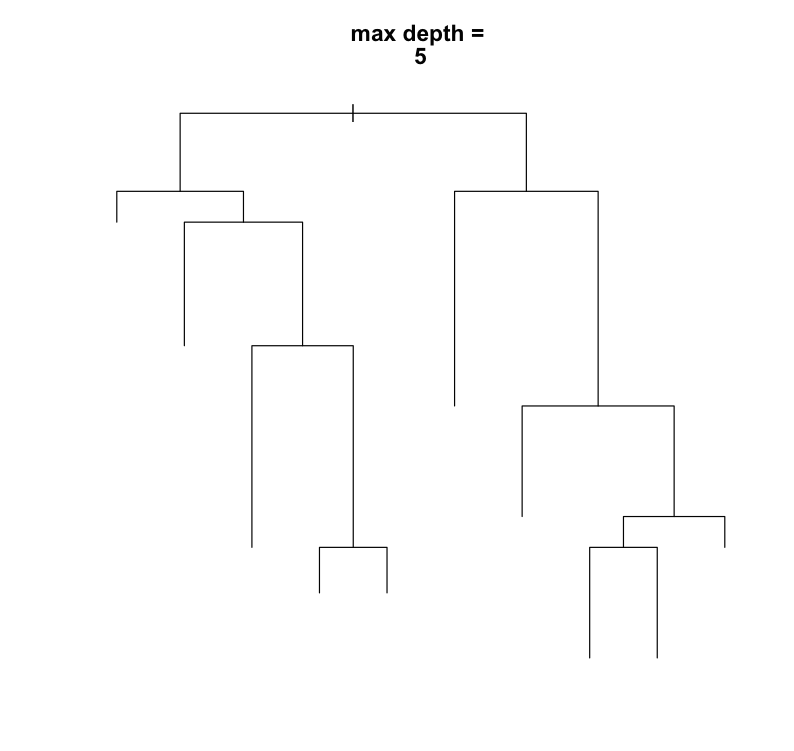
\includegraphics[scale=0.25]{images/mdepth=5}
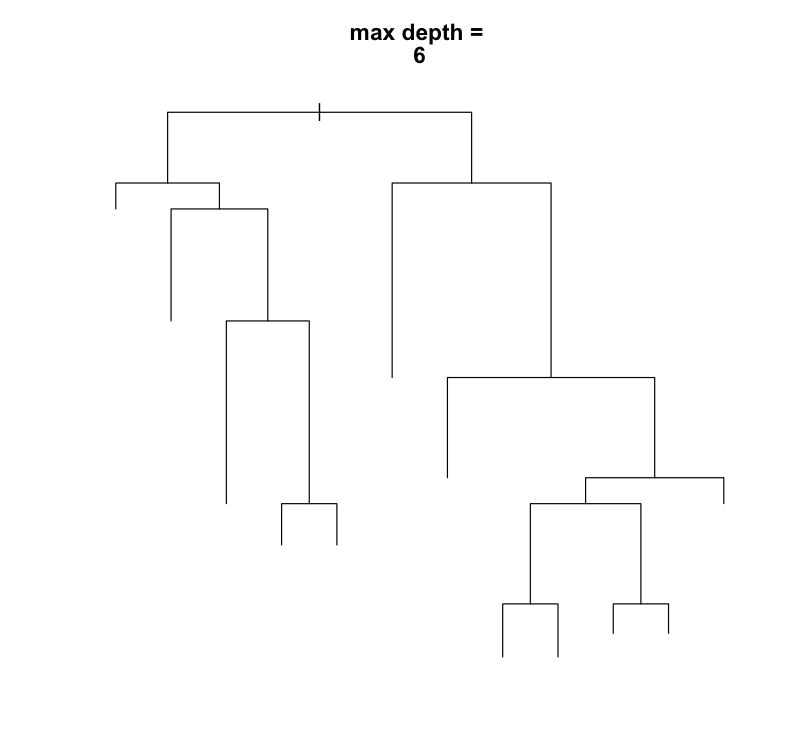
\includegraphics[scale=0.25]{images/mdepth=6}
\end{center}

\begin{Verbatim}
#e) Construct trees with minstplit = 1, cp = 10^{-2.0}, 10^{-2.1}, 
#   10^{-2.2}, ... , 10^{-2.9}, 10^{-3.0}, and store their 
#      training error
#      test error
#      number of nodes
#   in a matrix.
max_depth = seq(1, 10, 1)
train_error = rep(0, 10)
test_error = rep(0, 10)
n_nodes = rep(0, 10)

ct = 1
for(exp in seq(-2,-3,-0.1)){
  mycp = 10^exp  
  t_tree = rpart(as.factor(class)~.,traindata, 
                 control=rpart.control(minsplit=1, cp=mycp))
  plot(t_tree, main=c("cp = ", mycp))
  n_nodes[ct] = dim(t_tree$frame)[1]

  pred_t_tree = predict(t_tree, newdata = traindata, type='class')
  t_matrix = table(traindata$class, pred_t_tree)
  t_accuracy = sum(diag(t_matrix)) / sum(t_matrix)

  train_error[ct] = 1 - t_accuracy

  pred_t_tree = predict(t_tree, newdata = testdata, type='class')
  t_matrix = table(testdata$class, pred_t_tree)
  t_accuracy = sum(diag(t_matrix)) / sum(t_matrix)

  test_error[ct] = 1 - t_accuracy
  max_depth[ct] = ct
  ct=ct + 1
}

ctrl2 <-data.frame(max_depth, train_error, test_error, n_nodes)
\end{Verbatim}

\begin{center}
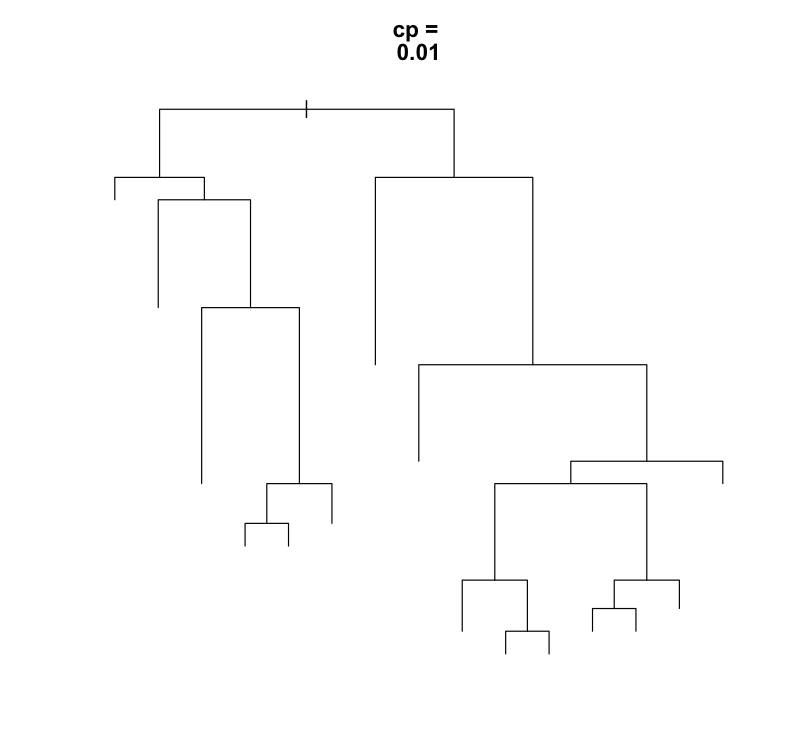
\includegraphics[scale=0.25]{images/ctrl1}
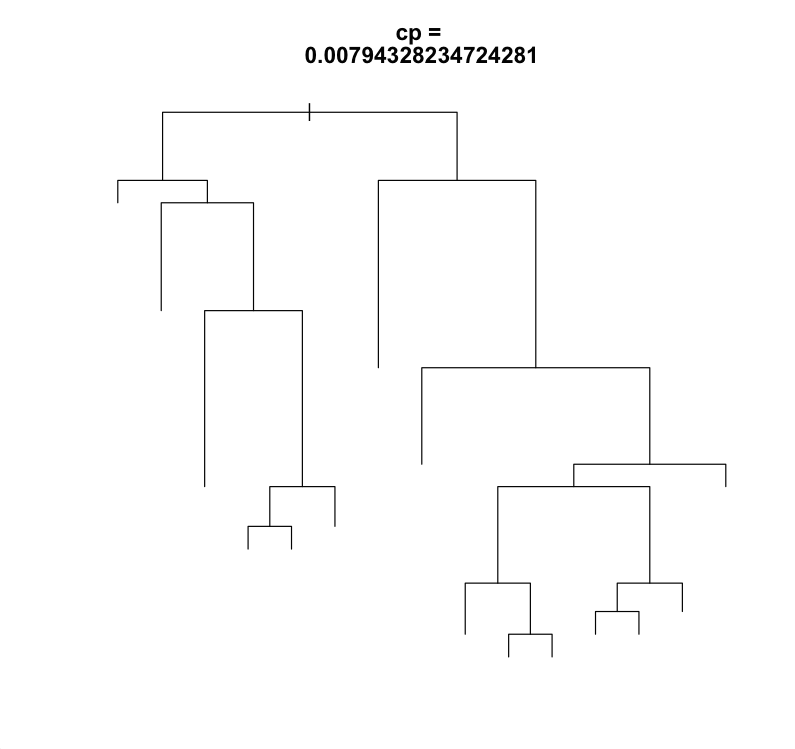
\includegraphics[scale=0.25]{images/ctrl2}
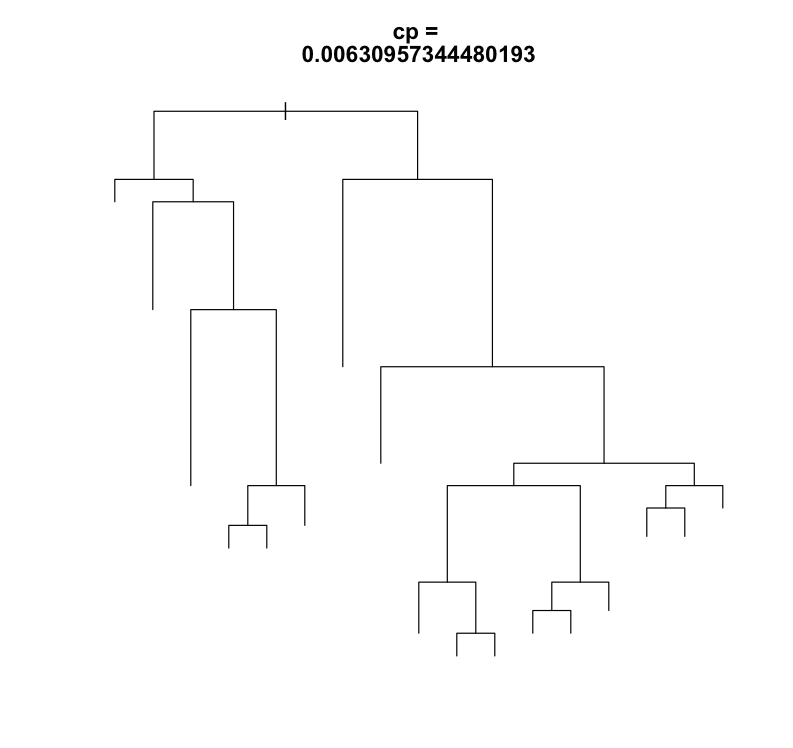
\includegraphics[scale=0.25]{images/ctrl3}
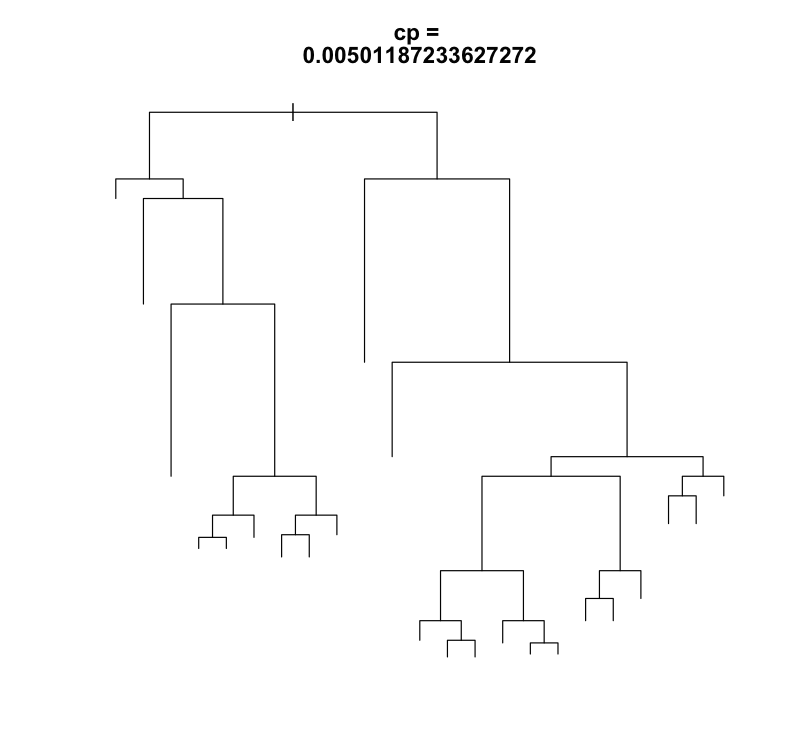
\includegraphics[scale=0.25]{images/ctrl4}
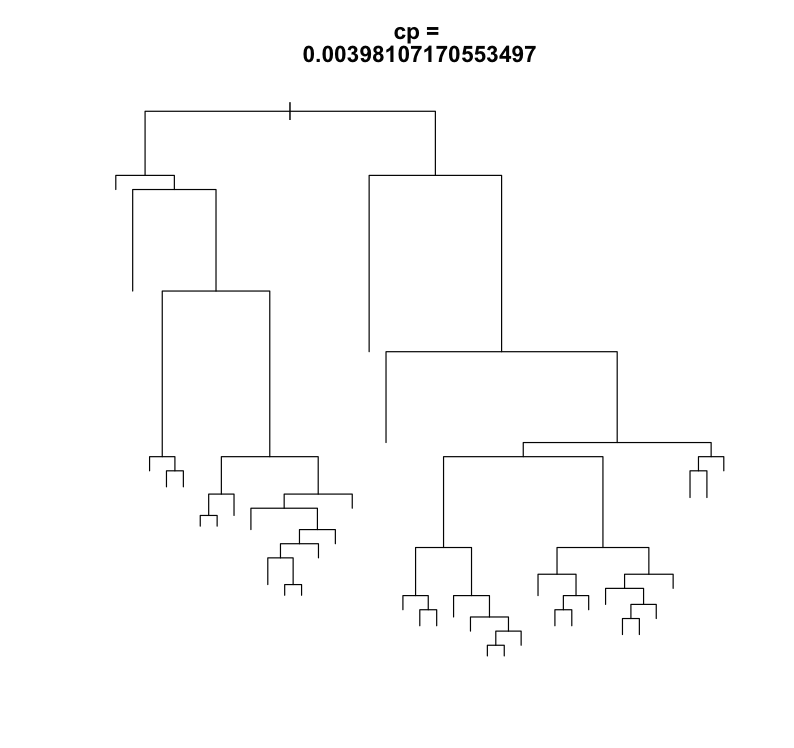
\includegraphics[scale=0.25]{images/ctrl5}
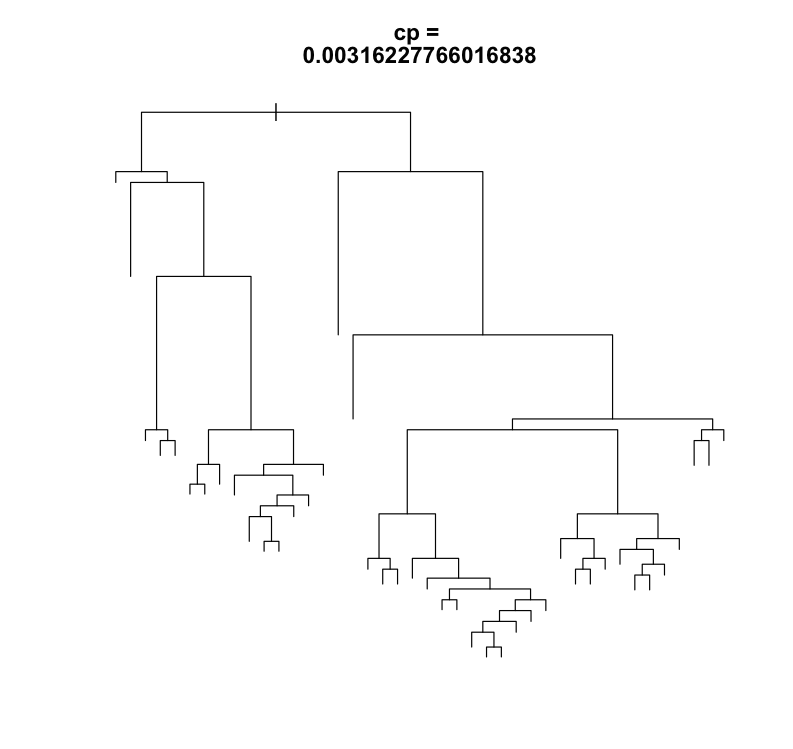
\includegraphics[scale=0.25]{images/ctrl6}
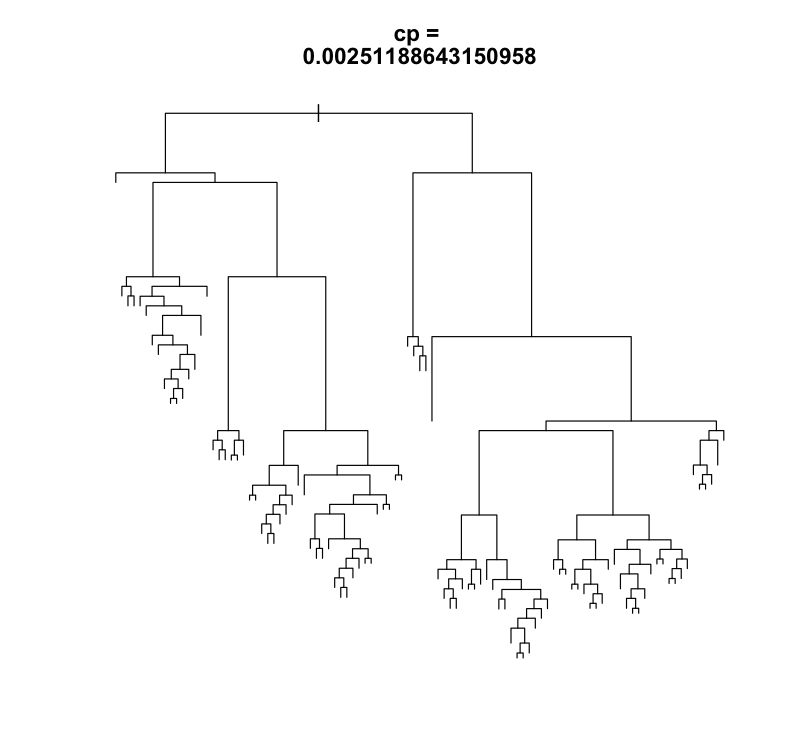
\includegraphics[scale=0.25]{images/ctrl7}
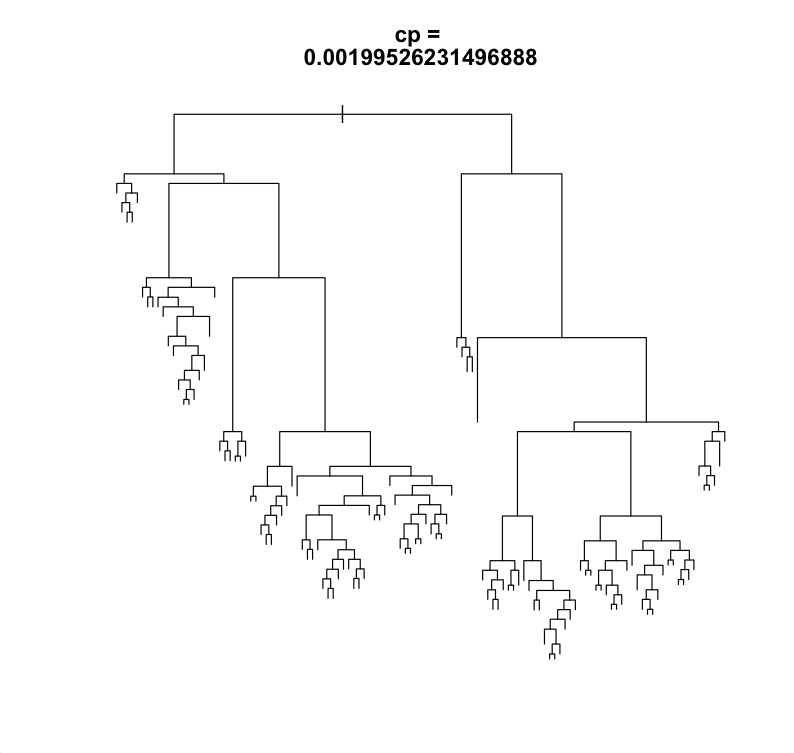
\includegraphics[scale=0.25]{images/ctrl8}
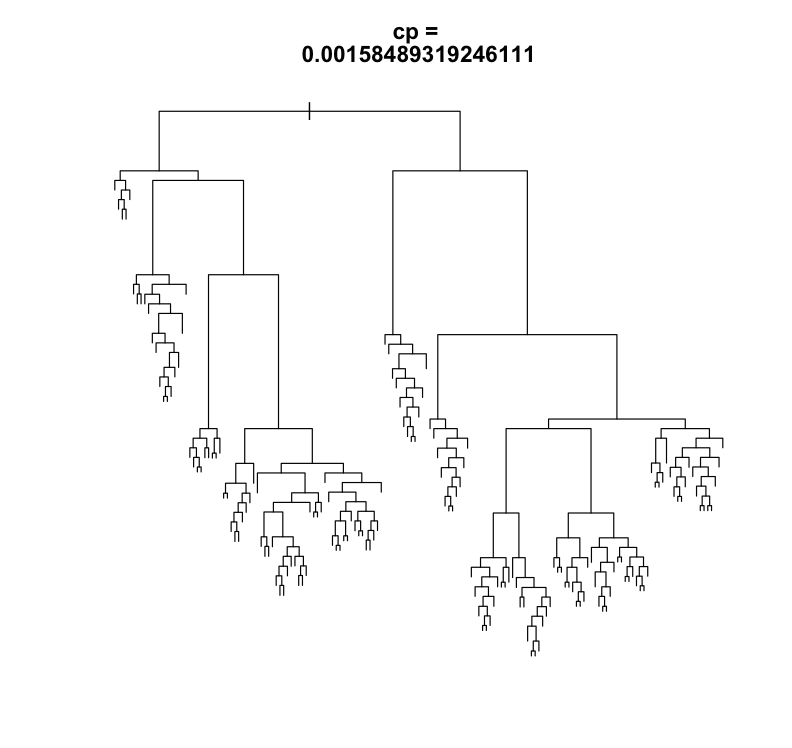
\includegraphics[scale=0.25]{images/ctrl9}
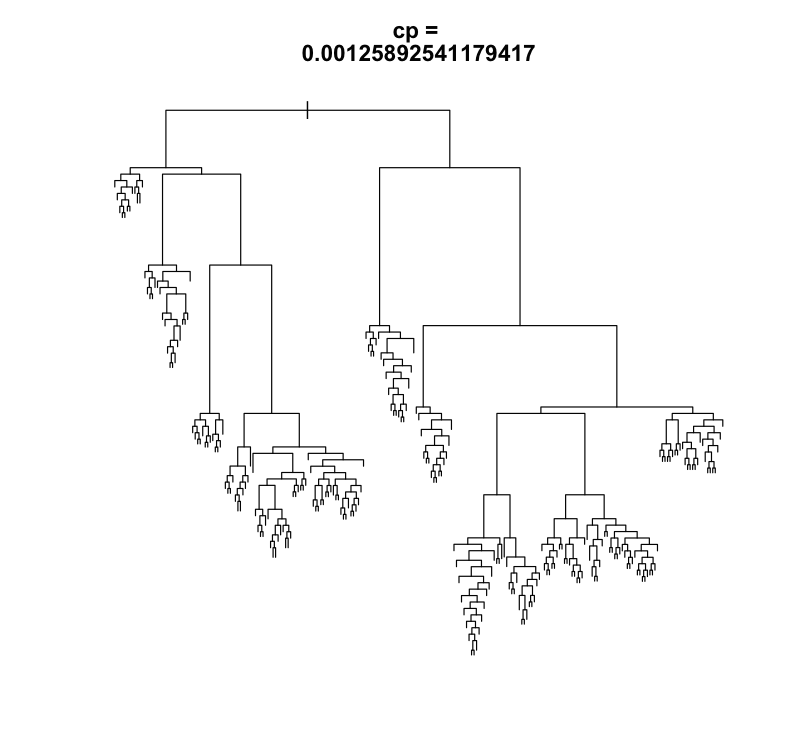
\includegraphics[scale=0.25]{images/ctrl10}
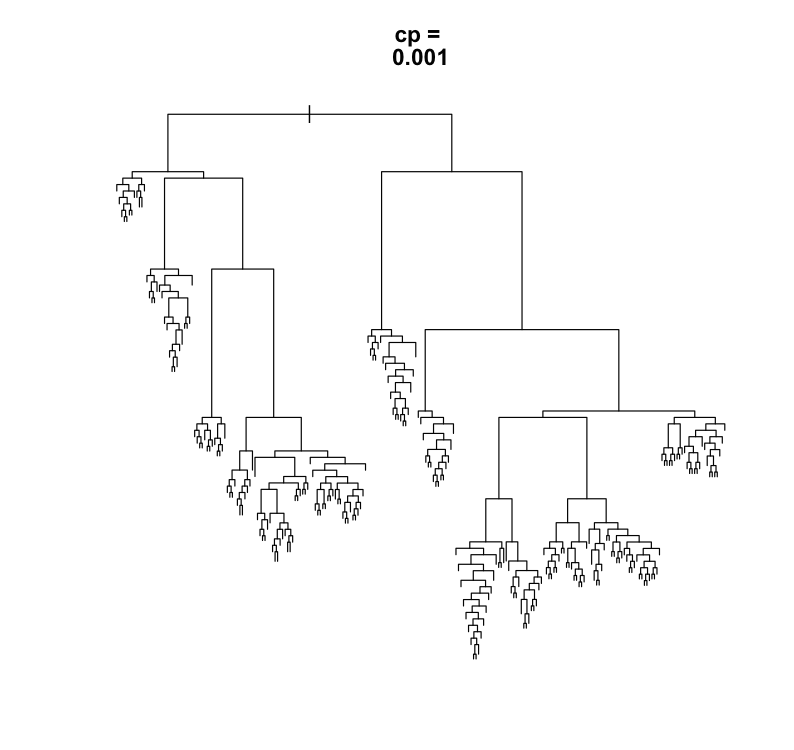
\includegraphics[scale=0.25]{images/ctrl11}
\end{center}

\begin{Verbatim}

#f) Use the information in this matrix to reproduce the plot of 
#   training/test error vs. number of nodes, as given on p. 54 of slides.
number_of_nodes = c(ctrl1$n_nodes, ctrl2$n_nodes)
error = c(ctrl1$train_error, ctrl2$train_error)
testing_error = c(ctrl1$test_error, ctrl2$test_error)

plot(number_of_nodes, error,type='l',col='black',ylim=c(0,max(testing_error)))
lines(number_of_nodes, testing_error,col='blue')
legend(0,0.1,c("Training error","Testing error"),col=c("black","blue"),lty=c(1,1))
\end{Verbatim}

\begin{center}
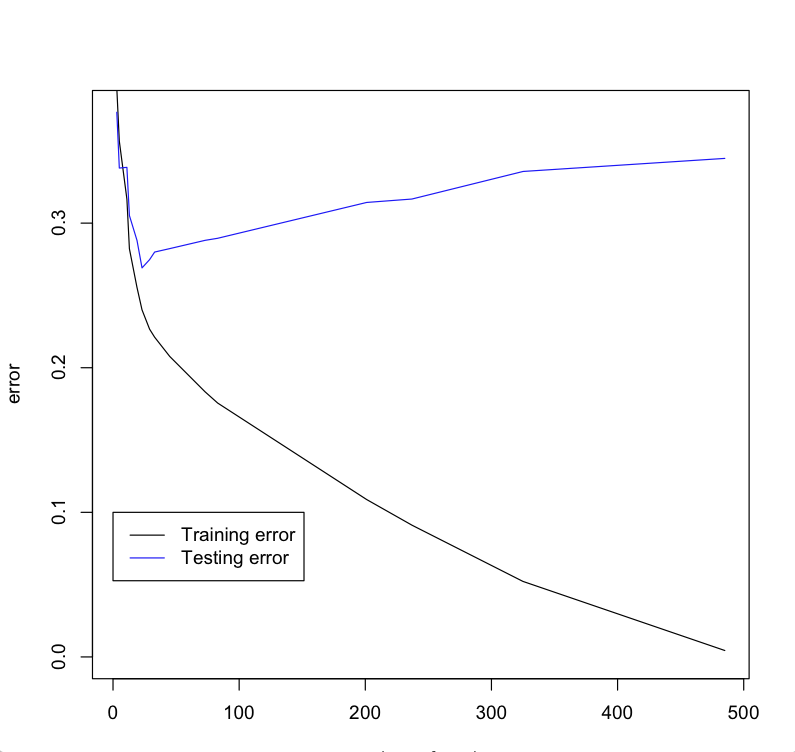
\includegraphics[scale=0.35]{images/trainvstest}
\end{center}

\begin{Verbatim}
#g) Let extree2 be the tree with minsplit = 1 and cp = 10^{-3}, and plot 
#   this tree.
#since this was the last instantiation of t_tree, can re-plot.
plot(t_tree)
\end{Verbatim}

\begin{center}
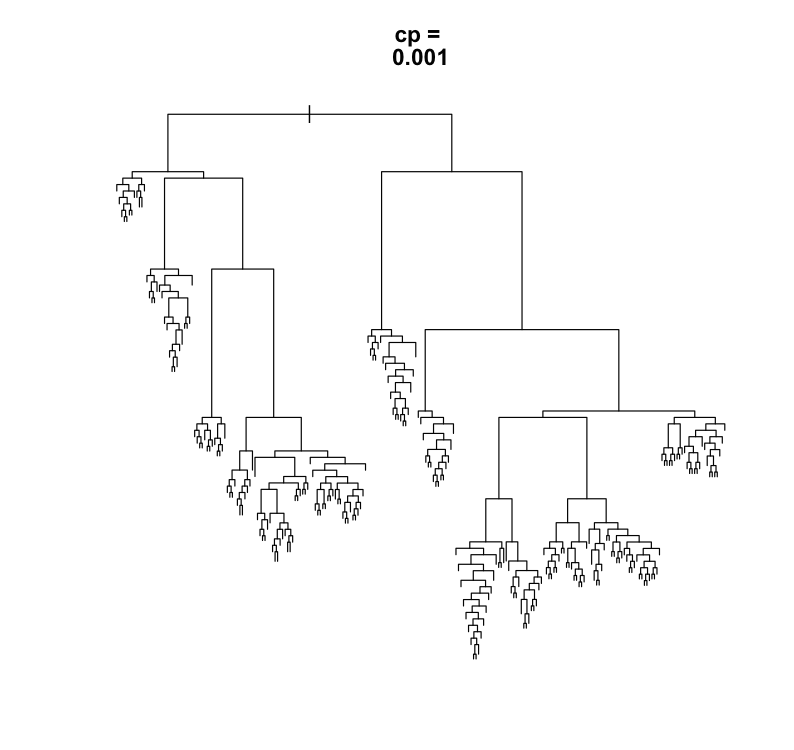
\includegraphics[scale=0.35]{images/ctrl11}
\end{center}

\begin{Verbatim}
#h)Use McNemar's test to determine if there is a statistically 
#  significant difference between the accuracies of extree and extree2
library(stats)
library(exact2x2)
accvector1 = (testdata$class == predict(extree, testdata, type='class'))
accvector2 = (testdata$class == predict(t_tree, testdata, type='class'))
mcnemartable = table(accvector1,accvector2)
mcnemar.exact(mcnemartable)

\end{Verbatim}
The $p-$value for the McNemar test was 2.2e-16. Thus there is a 
huge difference between the accuracies of the two trees.

\begin{Verbatim}
####################################################################
#3. write a function called zcritical that accepts inputs alpha and numtails
#   and returns z_alpha when numtails=1 and z_{alpha / 2} when numtails = 2.
#   Verify that zcritical(0.05, 2) = 1.96 and zcritical(0.05, 1) = 1.645. 
#   The qnorm function will be helpful on this problem. 
zcritical = function(alpha, numtails){
    if(numtails == 1){
    	z_alpha = qnorm(1 - alpha)
    }else if(numtails == 2){
    	z_alpha = qnorm(1 - (0.5 * alpha))
    }else{
    	print("Error in function zcritical: numtails not valid input")
    }
	return(z_alpha)
}

####################################################################
#4. Write a function called accuracyconfint that accepts inputs 
#   accuracy, n, and alpha
#   and returns the confidence interval for accuracy given on p. 62 of the 
#   slides. Use this function to find a confidence interval for the accuracy 
#   of extree.
accuracyconfint = function(accuracy, n, alpha){
  zalpha = zcritical(alpha, 2)
	confintlow = ((2 * n * accuracy) + (zalpha^2) - 
	              (zalpha * sqrt(zalpha^2 + 4*n*accuracy - 
                       4*n*(accuracy^2)))) / (2*(n + zalpha^2))
	confinthigh = ((2 * n * accuracy) + (zalpha^2) + 
                      (zalpha * sqrt(zalpha^2 + 4*n*accuracy - 
                       4*n*(accuracy^2)))) / (2*(n + zalpha^2))
    return(c(confintlow, confinthigh))
}
\end{Verbatim}

The confidence interval for extree is 
0.7359068 0.7726866

\begin{Verbatim}
####################################################################
#5. Randomly split kyphosis into about 70% training, 30% test data.

#a) Use rpart to fit a tree called ktree to the training data, and find 
#   the training and test error rates
attach(kyphosis)
num_traindata = ceiling(0.7 * nrow(kyphosis))
num_testdata = nrow(kyphosis) - num_traindata
k_traindata = kyphosis[sample(nrow(kyphosis), num_traindata),]
k_testdata <- kyphosis[which(!row.names(kyphosis) %in% row.names(k_traindata)), ]

ktree = rpart(as.factor(Kyphosis)~Age+Start+Number)

k_pred_extree = predict(ktree, newdata = k_traindata, type='class')
k_train_c_mat = table(k_traindata$Kyphosis, k_pred_extree)
k_train_accuracy = sum(diag(k_train_c_mat)) / sum(k_train_c_mat)

k_pred_extree = predict(ktree, newdata = k_testdata, type='class')
k_test_c_mat = table(k_testdata$Kyphosis, k_pred_extree)
k_test_accuracy = sum(diag(k_test_c_mat)) / sum(k_test_c_mat)
k_trainerror = 1 - k_train_accuracy
k_testerror = 1 - k_test_accuracy
\end{Verbatim}
The value of k$\_$trainerror for this problem is 0.122807, and the value of 
k$\_$testerror is 0.25.
\begin{Verbatim}

#b) Find an exact binomial confidence interval for the accuracy of ktree.
train_exact_acc = binom.test(k_trainerror*num_traindata, num_traindata)
test_exact_acc = binom.test(k_testerror*num_testdata, num_testdata)
\end{Verbatim}

The exact binomial confidence interval for ktree with traindata is
( 0.05082894, 0.23679500)

The exact binomial confidence interval for ktree with testdata is 
(0.09773041, 0.46711280)



\end{document}
